\documentclass[12pt,a4paper,oneside]{article}

% ----------------------------- Codificacao e idioma -----------------------
\usepackage[T1]{fontenc}
\usepackage[utf8]{inputenc}
\usepackage{babel}
\babelprovide[main,import]{portuguese} % locale moderno (ini) -> hifenizacao PT
\usepackage{mathptmx}                 % fonte serifada tipo Times (ABNT)

% ----------------------------- Layout / margens ABNT ----------------------
\usepackage[a4paper,left=3cm,top=3cm,right=2cm,bottom=2cm]{geometry}
\usepackage{setspace}                 % espacamento 1,5
\usepackage{indentfirst}              % recuo na 1a linha apos titulo
\usepackage{ragged2e}

% ----------------------------- Recursos -----------------------------------
\usepackage{graphicx}
\graphicspath{{../imagens/}}
\usepackage{amsmath,amssymb}
\usepackage{booktabs}
\usepackage{array}
\usepackage{caption}
\usepackage{float}
\usepackage{enumitem}
\usepackage{xcolor}
\usepackage{titlesec}
\usepackage[hidelinks]{hyperref}
\usepackage{xurl}                     % permite quebra de URLs longas

% ----------------------------- Nomes em portugues -------------------------
\AtBeginDocument{%
  \renewcommand{\figurename}{Figura}%
  \renewcommand{\tablename}{Tabela}%
  \renewcommand{\contentsname}{SUMÁRIO}%
  \renewcommand{\refname}{REFERÊNCIAS}%
  \renewcommand{\abstractname}{RESUMO}%
}

% ----------------------------- Estilo de titulos (ABNT NBR 6024) ----------
\titleformat{\section}{\normalfont\bfseries\large}{\thesection}{0.6em}{\MakeUppercase}
\titleformat{\subsection}{\normalfont\bfseries\normalsize}{\thesubsection}{0.6em}{}
\titlespacing*{\section}{0pt}{1.2\baselineskip}{0.6\baselineskip}
\titlespacing*{\subsection}{0pt}{1.0\baselineskip}{0.4\baselineskip}

% legendas
\captionsetup{font=small,labelfont=bf,justification=centering}

% espacamento geral
\onehalfspacing
\setlength{\parindent}{1.25cm}
\justifying
\emergencystretch=2em   % evita pequenos estouros de linha em texto justificado

% ambiente para referencias ABNT (alinhado a esquerda, espaco simples)
\newenvironment{referencias}{%
  \begin{spacing}{1.0}\setlength{\parindent}{0pt}\setlength{\parskip}{12pt}%
  \sloppy\emergencystretch=3em\RaggedRight}{%
  \end{spacing}}

\begin{document}

% =========================================================================
% CAPA
% =========================================================================
\begin{titlepage}
\centering
{\large FIAP — FACULDADE DE INFORMÁTICA E ADMINISTRAÇÃO PAULISTA\par}
\vspace{0.4cm}
{\normalsize Engenharia de Software\par}
\vspace{3.5cm}

{\large\bfseries LINCOLN SIMÃO PEREIRA — RM 567284\par}
{\large\bfseries MIGUEL SILVA BEZERRA — RM 566763\par}
{\large\bfseries NICOLAS SAKAUE NISHIMURA — RM 567752\par}

\vspace{3.5cm}
{\LARGE\bfseries MODELAGEM DE IMAGENS DE SATÉLITE\\[0.25cm]
POR TRANSFORMAÇÕES LINEARES:\\[0.25cm]
MONITORAMENTO DO DESMATAMENTO\\[0.25cm]
NA INDÚSTRIA ESPACIAL\par}

\vfill
{\normalsize Disciplina: Modelagem Matemática e Computacional\par}
{\normalsize Professor: Igor Gimenes Cesca\par}
\vspace{1.5cm}
{\normalsize SÃO PAULO\par}
{\normalsize 2026\par}
\end{titlepage}

% =========================================================================
% RESUMO
% =========================================================================
\thispagestyle{empty}
\begin{center}\textbf{RESUMO}\end{center}
\begin{spacing}{1.0}\noindent
A indústria espacial gera, por meio de satélites de observação da Terra,
grandes volumes de dados que apoiam decisões em sustentabilidade, agronegócio
e meio ambiente. Este trabalho modela imagens orbitais multiespectrais como
matrizes e emprega \emph{transformações lineares} da Álgebra Linear para
monitorar o avanço do desmatamento em uma área florestal. São definidas como
variáveis de entrada as quatro bandas espectrais de cada pixel (azul, verde,
vermelho e infravermelho próximo). Sobre esses dados aplicam-se quatro
transformações lineares matriciais: (i) uma transformação espectral
$y = M\,p$ que separa as componentes de brilho, verdor e umidade; (ii) uma
transformação geométrica afim $W = R(\theta)\,S$ para registro (alinhamento)
de imagens de datas distintas; (iii) um realce linear de contraste
$g(x) = \alpha x + \beta$; e (iv) a detecção de mudança por subtração
matricial $\Delta = G(t_2) - G(t_1)$. A partir de uma base de dados sintética,
porém verossímil, em duas datas (2019 e 2024), o método identificou perda de
cobertura vegetal de aproximadamente $13{,}3\%$ da área monitorada,
equivalente a cerca de $64{,}5$ ha, demonstrando como operações matriciais
elementares sustentam aplicações reais de sensoriamento remoto.
\par\vspace{0.4cm}
\noindent\textbf{Palavras-chave:} Álgebra Linear. Transformação Linear.
Sensoriamento Remoto. Processamento de Imagens. Desmatamento.
\end{spacing}

\newpage
% =========================================================================
% SUMARIO
% =========================================================================
\thispagestyle{empty}
\tableofcontents
\newpage

\setcounter{page}{1}
\pagestyle{plain}

% =========================================================================
\section{Introdução}
% =========================================================================
A exploração espacial impulsiona uma nova corrida tecnológica com impacto
direto em setores como sustentabilidade, mobilidade, agronegócio, comunicação
e inteligência artificial. Entre os produtos dessa indústria, os satélites de
observação da Terra destacam-se por fornecer, de forma contínua e em escala
global, imagens que registram o estado da superfície terrestre. Cada imagem
captada é, do ponto de vista computacional, uma matriz de números: a cada
posição $(i,j)$ corresponde um pixel, e a cada pixel associam-se valores de
reflectância em diferentes faixas do espectro eletromagnético.

Essa representação matricial torna a Álgebra Linear a linguagem natural para
processar imagens de satélite. Operações como combinar bandas espectrais,
alinhar imagens de datas diferentes, realçar contraste ou comparar duas cenas
podem ser escritas como \emph{transformações lineares} --- isto é, funções
$T:\mathbb{R}^n \to \mathbb{R}^m$ representáveis por matrizes. Este trabalho
explora exatamente essa ponte entre teoria e aplicação, escolhendo um problema
ambiental concreto e resolvendo-o por meio de transformações matriciais.

O objetivo geral é demonstrar como transformações lineares aplicadas a imagens
de satélite permitem monitorar o desmatamento. Como objetivos específicos,
busca-se: (a) definir as variáveis de entrada do problema; (b) formular as
transformações lineares matriciais adequadas; (c) construir uma base de dados
verossímil; e (d) interpretar os resultados obtidos.

% =========================================================================
\section{Definição do problema}
% =========================================================================
O problema real escolhido é o \textbf{monitoramento do desmatamento em áreas
florestais} a partir de imagens de satélite. Trata-se de uma aplicação
diretamente ligada à sustentabilidade: o acompanhamento periódico da cobertura
vegetal permite identificar a abertura de clareiras, estradas e áreas de
pastagem, subsidiando fiscalização ambiental e políticas públicas. No Brasil,
esse monitoramento é realizado operacionalmente pelo INPE em programas como o
PRODES e o DETER, ambos baseados em imagens orbitais.

A questão central que orientou a modelagem foi: \emph{como, a partir de duas
imagens da mesma região em datas diferentes, quantificar de forma automática a
perda de vegetação usando apenas operações de Álgebra Linear?} A resposta
proposta organiza-se em um fluxo de transformações lineares, detalhado na
Seção~\ref{sec:modelagem}.

% =========================================================================
\section{Fundamentação teórica}
% =========================================================================

\subsection{A imagem digital como matriz}
Uma imagem em tons de cinza de dimensões $m \times n$ é uma matriz
$A \in \mathbb{R}^{m\times n}$, em que o elemento $a_{ij}$ representa a
intensidade do pixel na linha $i$ e coluna $j$. Em imagens multiespectrais,
cada pixel carrega não um, mas $k$ valores --- um por banda espectral. Assim, a
cena completa pode ser vista como um \emph{tensor} $m\times n\times k$, ou,
equivalentemente, como uma coleção de $m\cdot n$ vetores
$p \in \mathbb{R}^{k}$, um por pixel.

\subsection{Transformações lineares e matrizes}
Uma função $T:\mathbb{R}^n \to \mathbb{R}^m$ é uma \emph{transformação linear}
quando preserva soma e multiplicação por escalar:
\begin{equation}
T(\alpha u + \beta v) = \alpha\,T(u) + \beta\,T(v),
\qquad \forall\, u,v \in \mathbb{R}^n,\ \forall\,\alpha,\beta\in\mathbb{R}.
\end{equation}
Todo $T$ desse tipo é representado por uma matriz $M \in \mathbb{R}^{m\times n}$
tal que $T(p) = M\,p$. As colunas de $M$ são justamente as imagens dos vetores
da base canônica, $M e_j = T(e_j)$. Esse é o resultado que permite traduzir
operações sobre imagens em multiplicações matriciais.

\subsection{Interpretação geométrica}
No plano, uma transformação linear deforma a base canônica
$\{e_1,e_2\}$ em dois novos vetores $\{Ae_1, Ae_2\}$. O quadrado unitário é
levado em um paralelogramo cuja área vale $|\det A|$; quando
$\det A = 0$, a transformação é singular (colapsa o plano em uma reta ou ponto)
e não admite inversa. A Figura~\ref{fig:vetores} ilustra a transformação
$A = R(\theta)\,S$, composição de uma rotação de $25^\circ$ com uma escala
$\operatorname{diag}(1{,}6;\,0{,}9)$, para a qual $\det A = 1{,}44$.

\begin{figure}[H]
\centering
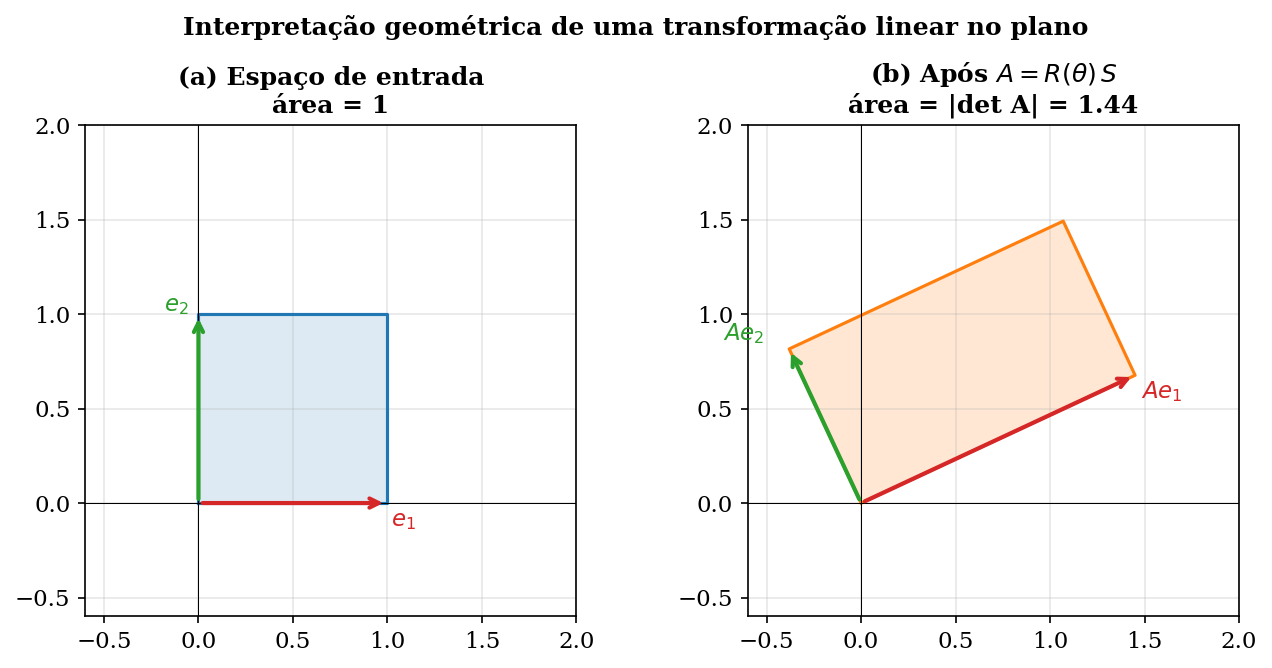
\includegraphics[width=0.95\textwidth]{fig02_algebra_vetores.png}
\caption{Interpretação geométrica de uma transformação linear no plano: o
quadrado unitário (área 1) é levado em um paralelogramo de área $|\det A|$.}
\label{fig:vetores}
\end{figure}

% =========================================================================
\section{Modelagem matemática}\label{sec:modelagem}
% =========================================================================
A modelagem organiza-se em um fluxo de quatro transformações lineares
aplicadas às imagens, descritas a seguir.

\subsection{Variáveis de entrada}
Para cada pixel define-se o vetor de bandas espectrais
\begin{equation}
p = \begin{bmatrix} B \\ G \\ R \\ \mathrm{NIR} \end{bmatrix} \in \mathbb{R}^{4},
\end{equation}
em que $B$, $G$, $R$ e $\mathrm{NIR}$ são as reflectâncias (normalizadas em
$[0,1]$) nas faixas do azul, verde, vermelho e infravermelho próximo. Essas
quatro bandas são as variáveis de entrada do modelo e correspondem às faixas
efetivamente captadas por satélites como o Sentinel-2.

\subsection{Transformação espectral linear}
A primeira transformação combina linearmente as bandas para separar
informações físicas da cena. Inspirada na transformação \emph{Tasseled Cap} do
sensoriamento remoto, ela é definida por $y = M\,p$, com
\begin{equation}
\underbrace{\begin{bmatrix} \text{Brilho}\\ \text{Verdor}\\ \text{Umidade}\end{bmatrix}}_{y\,\in\,\mathbb{R}^3}
=
\underbrace{\begin{bmatrix}
\phantom{-}0{,}33 & \phantom{-}0{,}34 & \phantom{-}0{,}33 & \phantom{-}0{,}49\\
-0{,}27 & -0{,}22 & -0{,}55 & \phantom{-}0{,}72\\
\phantom{-}0{,}19 & \phantom{-}0{,}31 & \phantom{-}0{,}24 & -0{,}61
\end{bmatrix}}_{M\,\in\,\mathbb{R}^{3\times 4}}
\underbrace{\begin{bmatrix} B\\ G\\ R\\ \mathrm{NIR}\end{bmatrix}}_{p}.
\end{equation}
A componente \textbf{Verdor} ($G$) é o indicador de vegetação: como pesa
positivamente o NIR e negativamente as bandas visíveis, assume valores altos
em floresta sadia e baixos em solo exposto. A Figura~\ref{fig:espectral}
mostra a separação das três componentes na cena de 2024.

\begin{figure}[H]
\centering
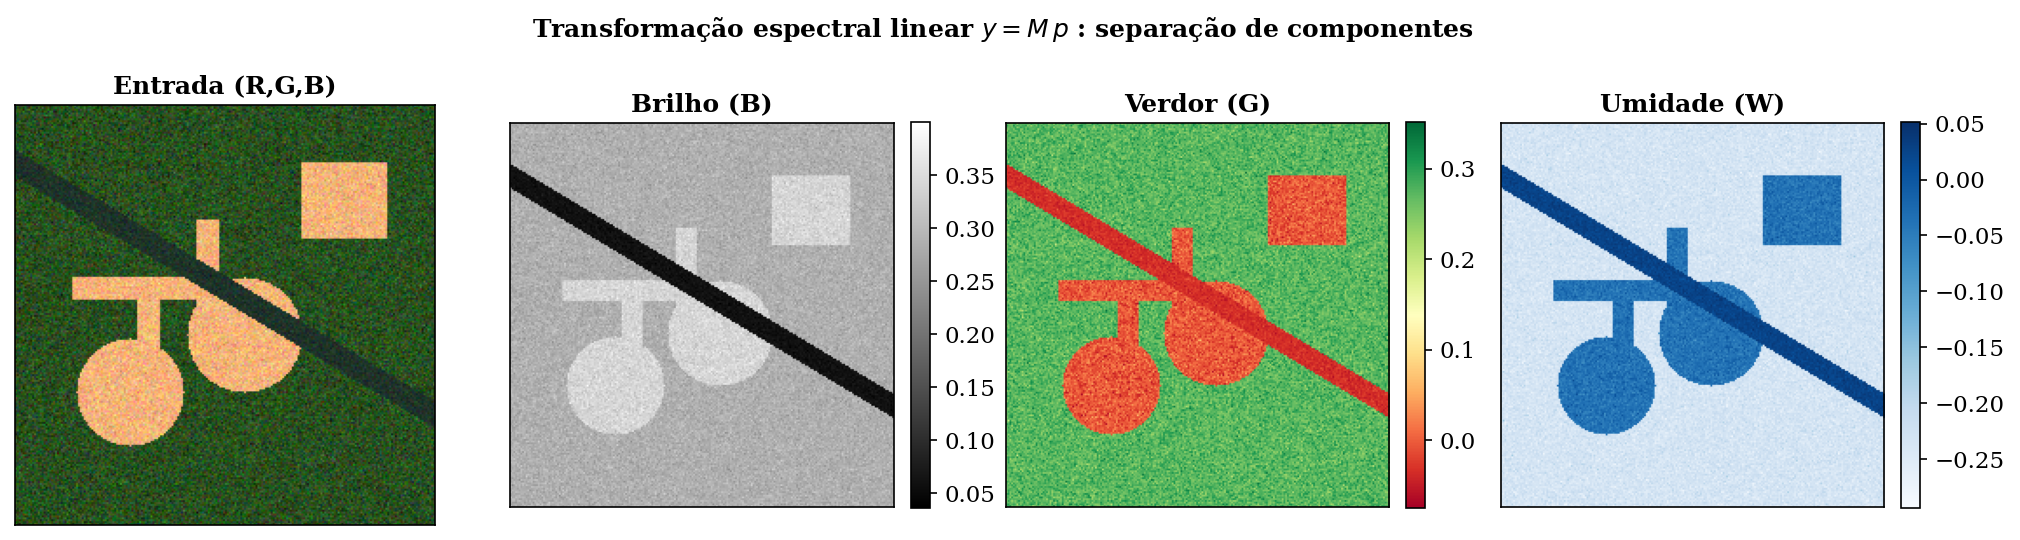
\includegraphics[width=\textwidth]{fig04_transformacao_espectral.png}
\caption{Transformação espectral linear $y = M\,p$ aplicada à cena de 2024.
O canal Verdor evidencia as áreas desmatadas (tons avermelhados).}
\label{fig:espectral}
\end{figure}

\subsection{Transformação geométrica: registro de imagens}
Imagens de datas distintas raramente estão perfeitamente alinhadas, devido a
variações de órbita e de ângulo de visada do satélite. O alinhamento (registro)
é obtido por uma transformação afim sobre as coordenadas dos pixels. Em
coordenadas homogêneas:
\begin{equation}
\begin{bmatrix} x'\\ y'\\ 1 \end{bmatrix}
=
\begin{bmatrix}
s_x\cos\theta & -s_y\sin\theta & t_x\\
s_x\sin\theta & \phantom{-}s_y\cos\theta & t_y\\
0 & 0 & 1
\end{bmatrix}
\begin{bmatrix} x\\ y\\ 1 \end{bmatrix},
\end{equation}
em que $R(\theta)$ é a rotação, $S=\operatorname{diag}(s_x,s_y)$ a escala e
$(t_x,t_y)$ a translação. Conhecida a deformação $W=R(\theta)S$ de uma
aquisição desalinhada, sua inversa $W^{-1}$ realinha a imagem à referência
(Figura~\ref{fig:geom}). A inversa existe porque $\det W \neq 0$.

\begin{figure}[H]
\centering
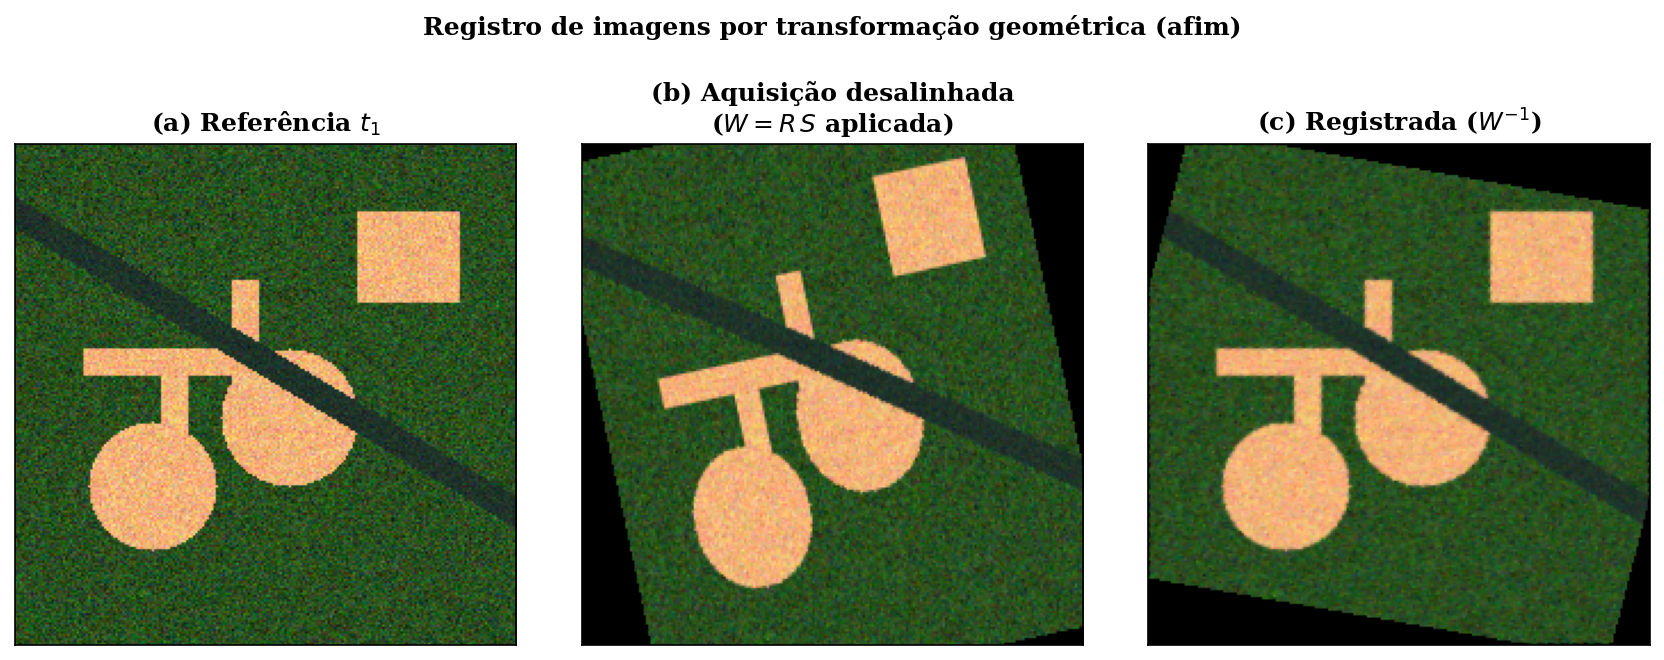
\includegraphics[width=\textwidth]{fig03_transformacao_geometrica.png}
\caption{Registro de imagens: a aquisição desalinhada (b) é realinhada à
referência (a) aplicando-se a transformação inversa $W^{-1}$ (c).}
\label{fig:geom}
\end{figure}

\subsection{Realce linear de contraste}
Para destacar as feições de interesse aplica-se a transformação afim escalar
$g(x) = \alpha x + \beta$ a cada valor de intensidade, com os parâmetros
ajustados pelos percentis $2\%$ e $98\%$ do histograma. No experimento
obteve-se $\alpha = 2{,}84$ e $\beta = 0{,}12$. A Figura~\ref{fig:realce}
compara o canal Verdor antes e depois do realce, evidenciando a expansão do
histograma para todo o intervalo dinâmico.

\begin{figure}[H]
\centering
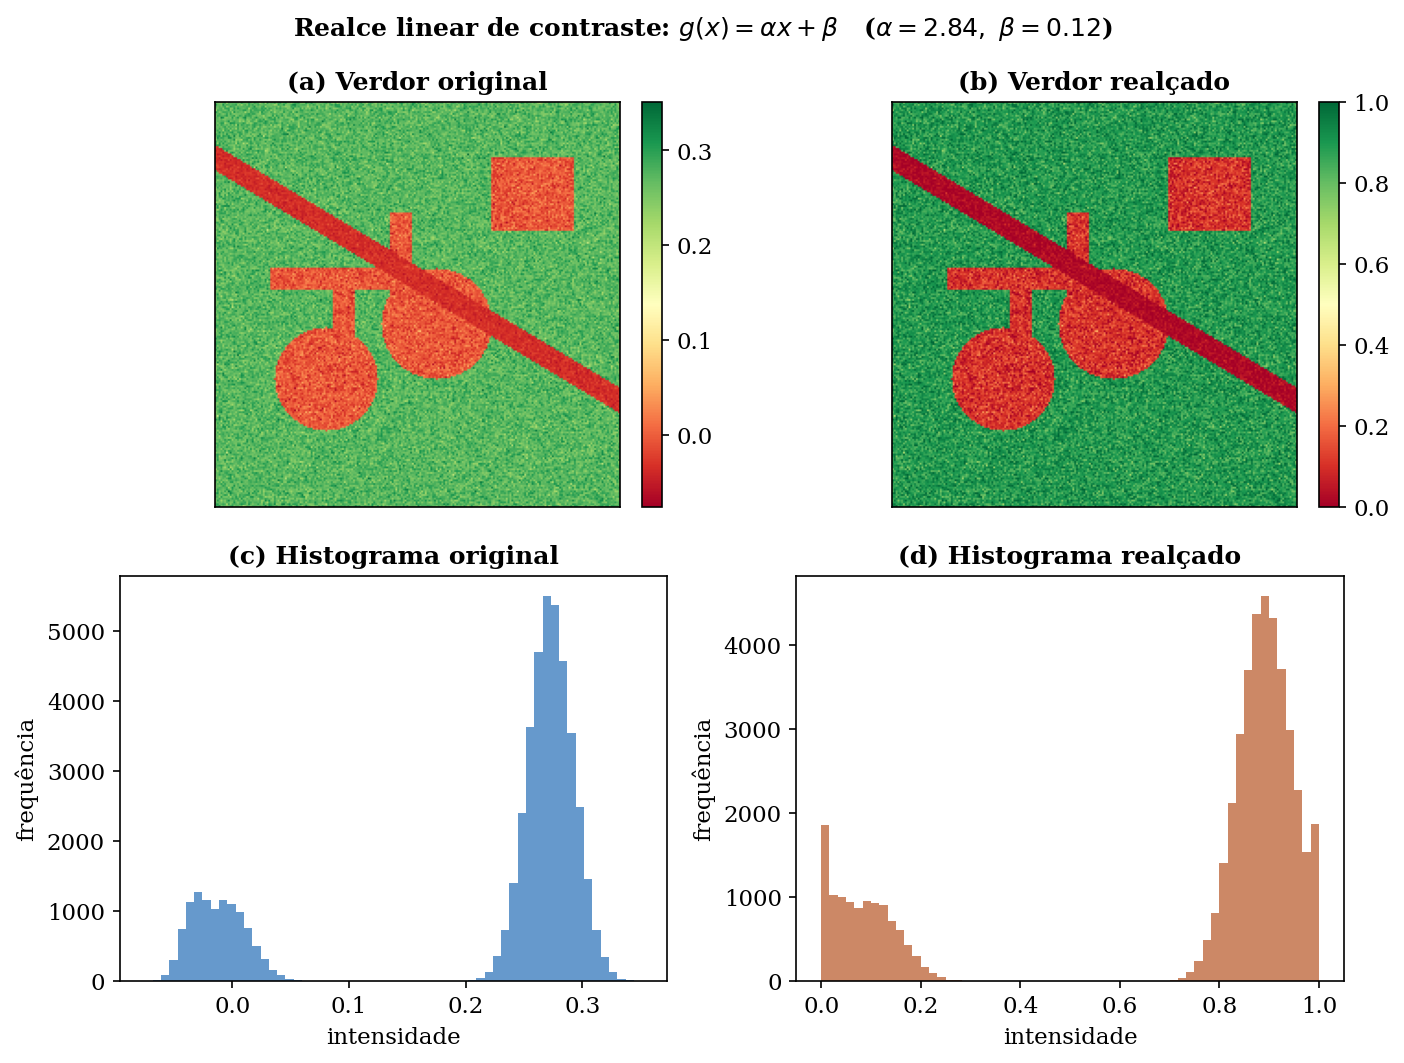
\includegraphics[width=0.85\textwidth]{fig05_realce_contraste.png}
\caption{Realce linear de contraste $g(x)=\alpha x + \beta$ aplicado ao canal
Verdor, com os respectivos histogramas.}
\label{fig:realce}
\end{figure}

\subsection{Detecção de mudança por subtração matricial}
Sejam $G(t_1)$ e $G(t_2)$ as matrizes do canal Verdor nas datas $t_1$ (2019) e
$t_2$ (2024), já registradas. A mudança é detectada pela subtração matricial
\begin{equation}
\Delta = G(t_2) - G(t_1),
\end{equation}
classificando-se como perda de vegetação todo pixel em que
$\Delta < -0{,}05$. Como a subtração de matrizes é uma operação linear, áreas
estáveis se anulam ($\Delta \approx 0$) e apenas as regiões efetivamente
alteradas permanecem, isolando o desmatamento ocorrido no período.

% =========================================================================
\section{Base de dados}
% =========================================================================
Por se tratar de um exercício de modelagem, construiu-se uma base de dados
sintética, porém verossímil, gerada em Python (\texttt{NumPy}). A cena tem
$220\times220$ pixels; adotando-se a resolução de $10\,$m por pixel
(compatível com o Sentinel-2), a área total monitorada equivale a $484$ ha.
A cada pixel atribuiu-se uma assinatura espectral média conforme a classe de
cobertura do solo, somada a ruído gaussiano (Tabela~\ref{tab:assin}).

\begin{table}[H]
\centering
\caption{Assinaturas espectrais médias (reflectância) por classe.}
\label{tab:assin}
\begin{tabular}{lcccc}
\toprule
\textbf{Classe} & \textbf{B} & \textbf{G} & \textbf{R} & \textbf{NIR}\\
\midrule
Floresta      & 0,04 & 0,09 & 0,05 & 0,46\\
Solo exposto  & 0,13 & 0,19 & 0,26 & 0,30\\
Água          & 0,05 & 0,06 & 0,04 & 0,02\\
\bottomrule
\end{tabular}
\end{table}

Foram geradas duas datas: em $t_1$ (2019) a floresta encontra-se quase intacta,
com um rio diagonal e pequenas clareiras pré-existentes; em $t_2$ (2024)
acrescentou-se um padrão de desmatamento em ``espinha de peixe'', típico da
abertura de estradas e pastagens (Figura~\ref{fig:rgb}). A base foi ainda
agregada em $25$ setores ($5\times5$), registrando-se para cada setor e data a
média das bandas, o índice de Verdor e a classe resultante, totalizando $50$
registros exportados em formato CSV.

\begin{figure}[H]
\centering
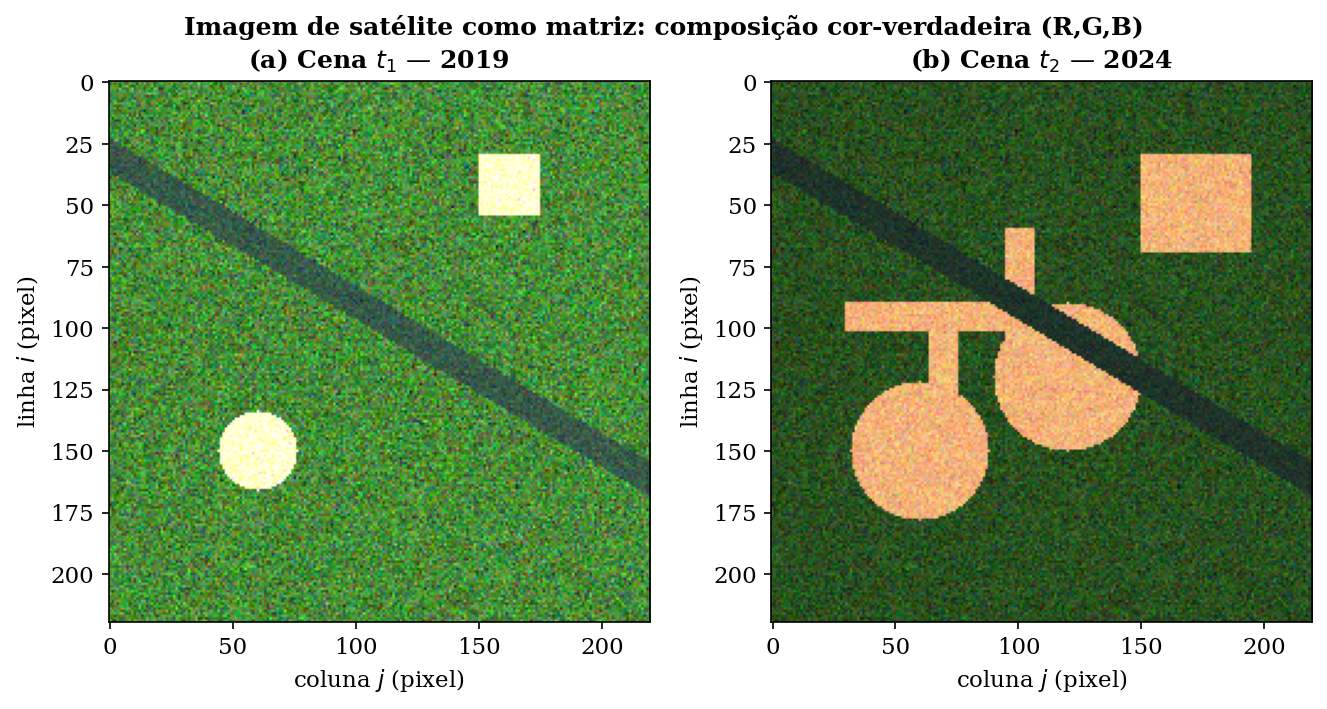
\includegraphics[width=0.9\textwidth]{fig01_cena_rgb.png}
\caption{Composição cor-verdadeira (R,G,B) da base sintética nas duas datas.}
\label{fig:rgb}
\end{figure}

% =========================================================================
\section{Resultados e discussão}
% =========================================================================
Aplicado o fluxo de transformações, a detecção de mudança apontou perda de
cobertura vegetal em $6\,448$ pixels, o que corresponde a $13{,}3\%$ da área
monitorada, ou aproximadamente $64{,}5$ ha desmatados entre 2019 e 2024
(Figura~\ref{fig:mudanca}). É importante notar que as clareiras já existentes
em $t_1$ \emph{não} foram contabilizadas: por se anularem na subtração, apenas
o desmatamento novo é destacado, o que valida o método.

\begin{figure}[H]
\centering
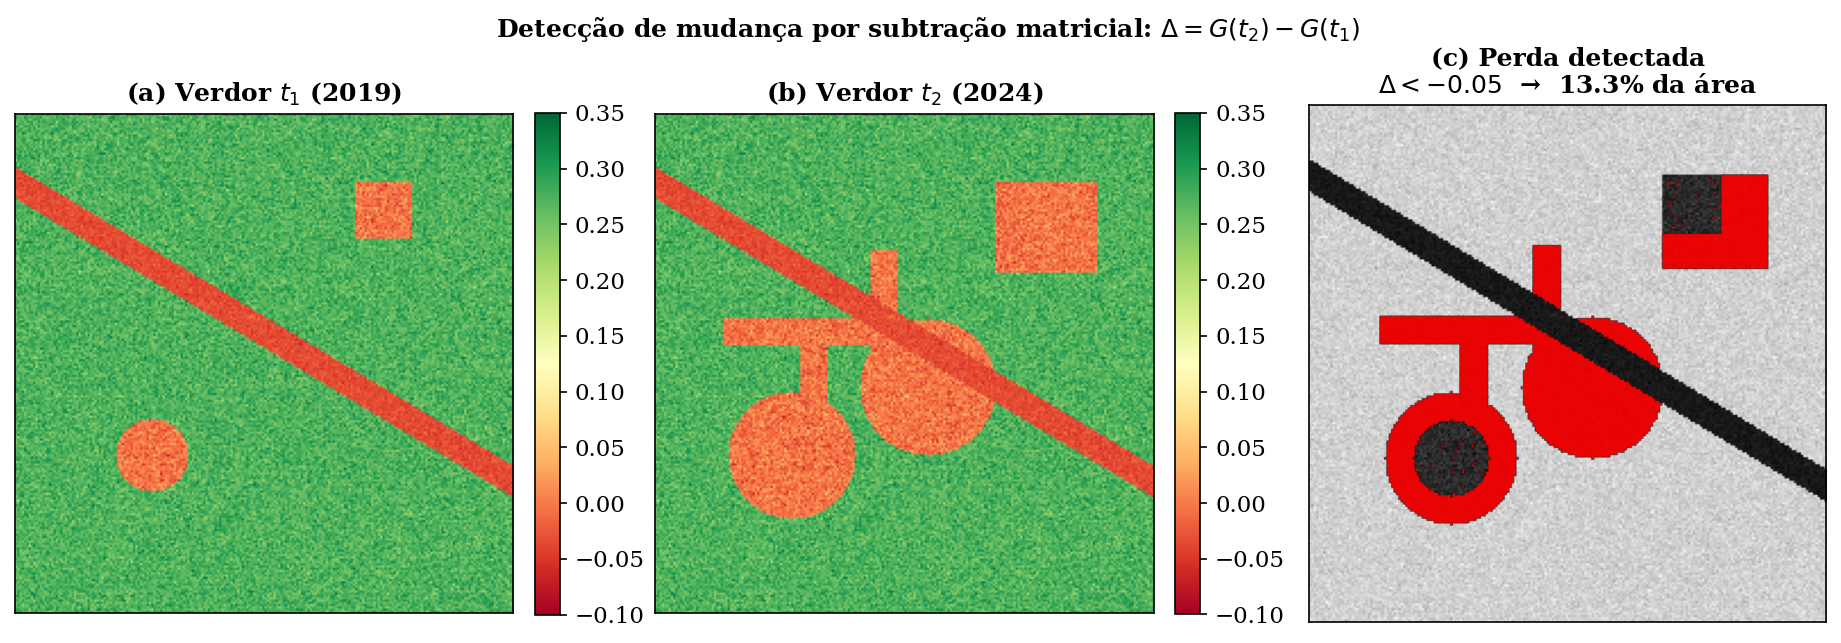
\includegraphics[width=\textwidth]{fig06_deteccao_mudanca.png}
\caption{Detecção de mudança $\Delta = G(t_2)-G(t_1)$. Em destaque (c), apenas
o desmatamento ocorrido no período; o rio é mascarado.}
\label{fig:mudanca}
\end{figure}

A análise por setores confirma o resultado em escala agregada. Dos $25$
setores, o número classificado como floresta caiu de $22$ (2019) para $18$
(2024). A Tabela~\ref{tab:setores} apresenta os quatro setores que mudaram de
classe, evidenciando o comportamento esperado: queda do Verdor, redução do NIR
(vegetação) e aumento do vermelho ($R$, solo exposto).

\begin{table}[H]
\centering
\caption{Setores que mudaram de classe entre 2019 e 2024.}
\label{tab:setores}
\begin{tabular}{lcccc}
\toprule
\textbf{Setor} & \textbf{Verdor 2019} & \textbf{Verdor 2024} & \textbf{NIR (19$\to$24)} & \textbf{R (19$\to$24)}\\
\midrule
S09 & 0,234 & 0,176 & 0,44 $\to$ 0,40 & 0,08 $\to$ 0,12\\
S12 & 0,273 & 0,121 & 0,46 $\to$ 0,37 & 0,05 $\to$ 0,17\\
S13 & 0,196 & 0,016 & 0,35 $\to$ 0,25 & 0,05 $\to$ 0,18\\
S14 & 0,192 & 0,146 & 0,34 $\to$ 0,32 & 0,05 $\to$ 0,08\\
\bottomrule
\end{tabular}
\end{table}

Os resultados mostram que operações matriciais elementares --- multiplicação
($y=Mp$), inversão ($W^{-1}$), escala afim ($\alpha x+\beta$) e subtração
($\Delta$) --- são suficientes para construir um detector de desmatamento
funcional. A principal limitação do estudo é o uso de dados sintéticos: em
imagens reais há nuvens, sombras e variação sazonal, que exigem etapas
adicionais de correção. Ainda assim, o núcleo algébrico do método permanece o
mesmo.

% =========================================================================
\section{Considerações finais}
% =========================================================================
O trabalho demonstrou, de ponta a ponta, como um problema ambiental relevante
--- o monitoramento do desmatamento --- pode ser modelado e resolvido por meio
de transformações lineares aplicadas a imagens de satélite. Tratando cada
imagem como uma matriz e cada pixel como um vetor de bandas, foi possível
formular transformações espectrais, geométricas e radiométricas, todas
expressas como multiplicações ou somas matriciais, culminando na detecção
quantitativa de perda de vegetação de $13{,}3\%$ da área.

Mais do que um exercício isolado, o estudo evidencia a importância da Álgebra
Linear como fundamento computacional da indústria espacial: os mesmos conceitos
de matrizes, determinantes e transformações que estruturam a teoria sustentam
aplicações concretas em sustentabilidade, agronegócio e inteligência
artificial. Como trabalho futuro, sugere-se a aplicação do fluxo a imagens
reais do Sentinel-2 e a incorporação de técnicas de classificação supervisionada.

% =========================================================================
\renewcommand{\refname}{REFERÊNCIAS}
\phantomsection
\addcontentsline{toc}{section}{REFERÊNCIAS}
\section*{REFERÊNCIAS}
% =========================================================================
\begin{referencias}
ANTON, Howard; RORRES, Chris. \textbf{Álgebra Linear com Aplicações}. 10. ed. Porto Alegre: Bookman, 2012.

BOLDRINI, José Luiz et al. \textbf{Álgebra Linear}. 3. ed. São Paulo: Harbra, 1986.

CRIST, Eric P.; CICONE, Richard C. A Physically-Based Transformation of Thematic Mapper Data: the TM Tasseled Cap. \textbf{IEEE Transactions on Geoscience and Remote Sensing}, v. GE-22, n. 3, p. 256-263, 1984.

GONZALEZ, Rafael C.; WOODS, Richard E. \textbf{Processamento Digital de Imagens}. 3. ed. São Paulo: Pearson, 2010.

INSTITUTO NACIONAL DE PESQUISAS ESPACIAIS (INPE). \textbf{Projeto PRODES: monitoramento do desmatamento da floresta amazônica brasileira por satélite}. Disponível em: \url{http://www.obt.inpe.br/prodes}. Acesso em: 29 maio 2026.

MENESES, Paulo Roberto; ALMEIDA, Tati de (Org.). \textbf{Introdução ao processamento de imagens de sensoriamento remoto}. Brasília: UnB/CNPq, 2012.
\end{referencias}

\end{document}
